\documentclass[a4paper]{article}

\usepackage[utf8]{inputenc}
\usepackage[dutch]{babel}
\usepackage{float}
\usepackage{subfig}
\usepackage{graphicx}


\begin{document}
	\section{Voorlopige resultaten}		
		Op dit moment kunnen we al effectief de foto gebruiksklaar maken voor de analyse ervan. Dit houdt in dat we alle pixels die niet tot de bloedklonter behoren wit kunnen maken en de afbeelding zodanig kunnen bijsnijden dat er geen overbodig geheugen ingenomen wordt door de afbeelding. In Figuur \ref{fig: voorna} wordt dit geïllustreerd.
		
		\begin{figure}[H]
			\centering
			\subfloat[Afbeelding van bloedklonter voor die bewerkt wordt]{{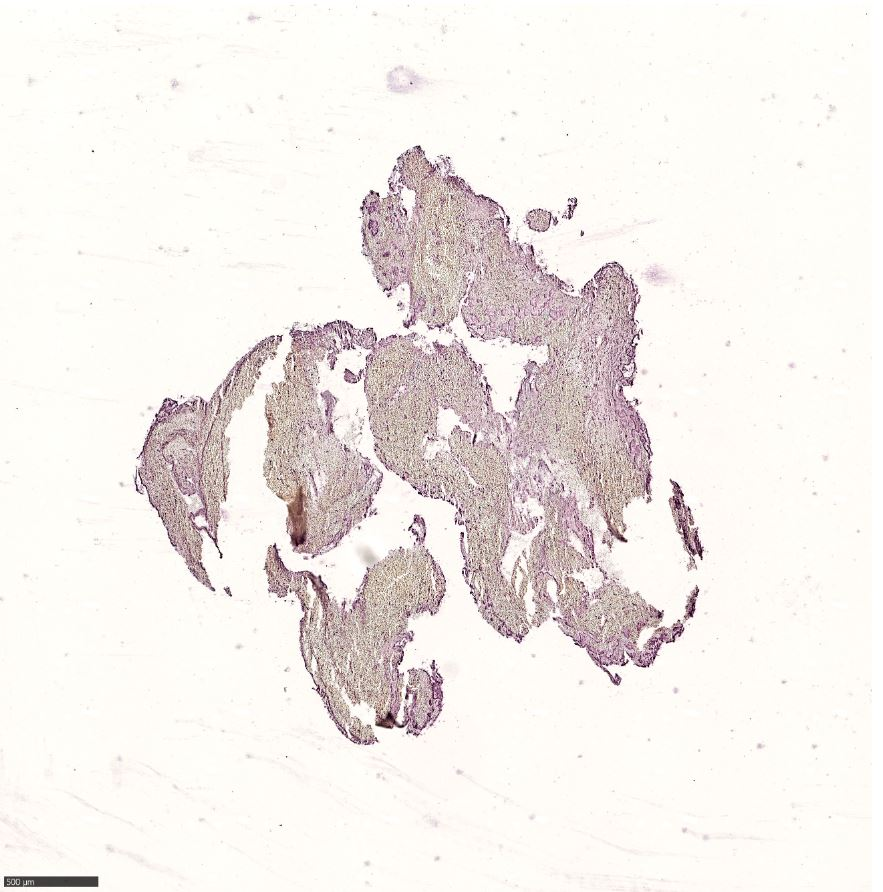
\includegraphics[width=4.5cm]{BloedklonterVoor.jpg}}}
			\qquad
			\subfloat[Bijgesneden afbeelding van de Bloedklonter met witte achtergrond ]{{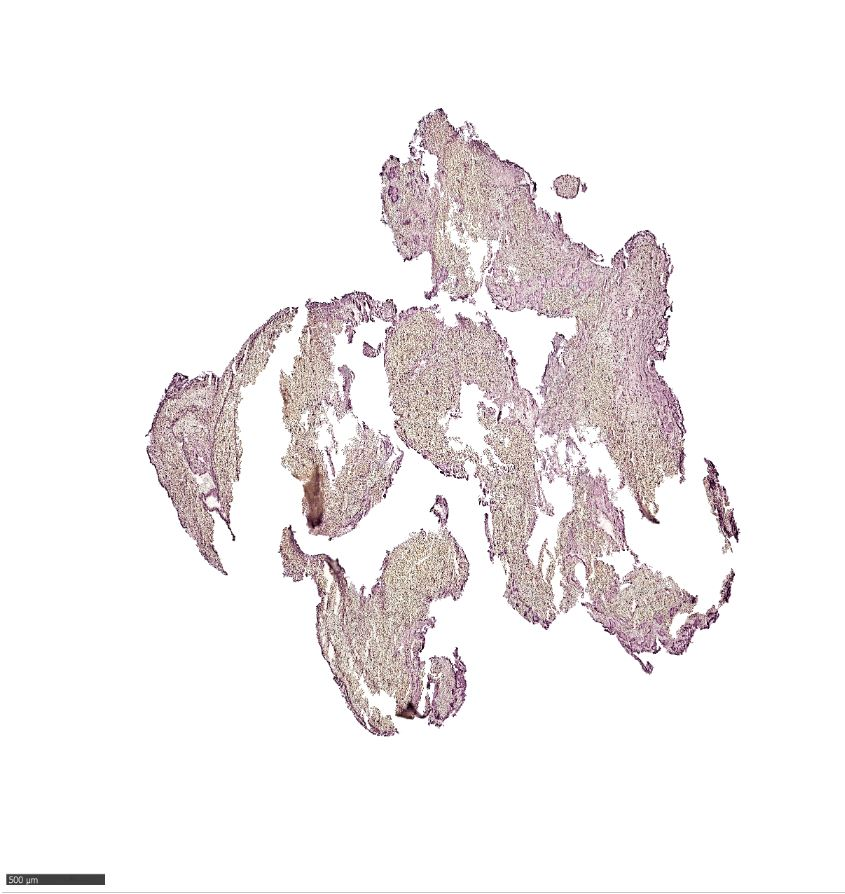
\includegraphics[width=4.5cm]{BloedklonterNa.jpg}}}

			\caption{Illustratie van hoe we de afbeelding gebruiksklaar maken voor de analyse ervan}
			\label{fig: voorna}
		\end{figure}
	
		Momenteel zijn we bezig met de implementatie van de kleurendetectie. We hebben hier al veel vooruitgang geboekt, maar de hij staat nog niet volledig op punt. Ook hebben we al even geëxperimenteerd met de app designer van Matlab. Hier willen we namelijk onze gebruiksvriendelijke applicatie in maken.
		
		Op basis van wat we nu al bereikt hebben, denken we dat dit project een succes kan worden en dat men het effectief zal kunnen gebruiken in het onderzoek naar de samenstelling van bloedklonters.
	
\end{document}